% --------------------------------------------------------------
% This is all preamble stuff that you don't have to worry about.
% Head down to where it says "Start here"
% --------------------------------------------------------------

\documentclass[12pt]{article}

\usepackage[margin=1in]{geometry}
\usepackage{amsmath,amsthm,amssymb}
\usepackage{graphicx} %This allows to include eps figures
\usepackage{subcaption}
\usepackage[section]{placeins}
\usepackage{layout}
\usepackage{etoolbox}
\usepackage{mathabx}
\usepackage{animate}
\usepackage{array}
% This is to include code
\usepackage{listings}
\usepackage{xcolor}
\definecolor{dkgreen}{rgb}{0,0.6,0}
\definecolor{gray}{rgb}{0.5,0.5,0.5}
\definecolor{mauve}{rgb}{0.58,0,0.82}
\lstdefinestyle{Python}{
    language        = Python,
    basicstyle      = \ttfamily,
    keywordstyle    = \color{blue},
    keywordstyle    = [2] \color{teal}, % just to check that it works
    stringstyle     = \color{green},
    commentstyle    = \color{red}\ttfamily
}

\newenvironment{conditions}
  {\par\vspace{\abovedisplayskip}\noindent\begin{tabular}{>{$}l<{$} @{${}={}$} l}}
  {\end{tabular}\par\vspace{\belowdisplayskip}}

\newcommand{\N}{\mathbb{N}}
\newcommand{\Z}{\mathbb{Z}}

\newenvironment{theorem}[2][Theorem]{\begin{trivlist}
\item[\hskip \labelsep {\bfseries #1}\hskip \labelsep {\bfseries #2.}]}{\end{trivlist}}
\newenvironment{lemma}[2][Lemma]{\begin{trivlist}
\item[\hskip \labelsep {\bfseries #1}\hskip \labelsep {\bfseries #2.}]}{\end{trivlist}}
\newenvironment{exercise}[2][Exercise]{\begin{trivlist}
\item[\hskip \labelsep {\bfseries #1}\hskip \labelsep {\bfseries #2.}]}{\end{trivlist}}
\newenvironment{reflection}[2][Reflection]{\begin{trivlist}
\item[\hskip \labelsep {\bfseries #1}\hskip \labelsep {\bfseries #2.}]}{\end{trivlist}}
\newenvironment{proposition}[2][Proposition]{\begin{trivlist}
\item[\hskip \labelsep {\bfseries #1}\hskip \labelsep {\bfseries #2.}]}{\end{trivlist}}
\newenvironment{corollary}[2][Corollary]{\begin{trivlist}
\item[\hskip \labelsep {\bfseries #1}\hskip \labelsep {\bfseries #2.}]}{\end{trivlist}}



\begin{document}

% --------------------------------------------------------------
%                         Start here
% --------------------------------------------------------------

%\renewcommand{\qedsymbol}{\filledbox}

\title{Assignment 4 - Appendix}%replace X with the appropriate number
\author{Nalet Meinen and Pascal Wyss\\ %replace with your name
Finite Element Analysis I
}
\maketitle

\section{Methods}

\begin{figure}[!htb]
  \centering
  \begin{subfigure}{.5\textwidth}
    \centering
    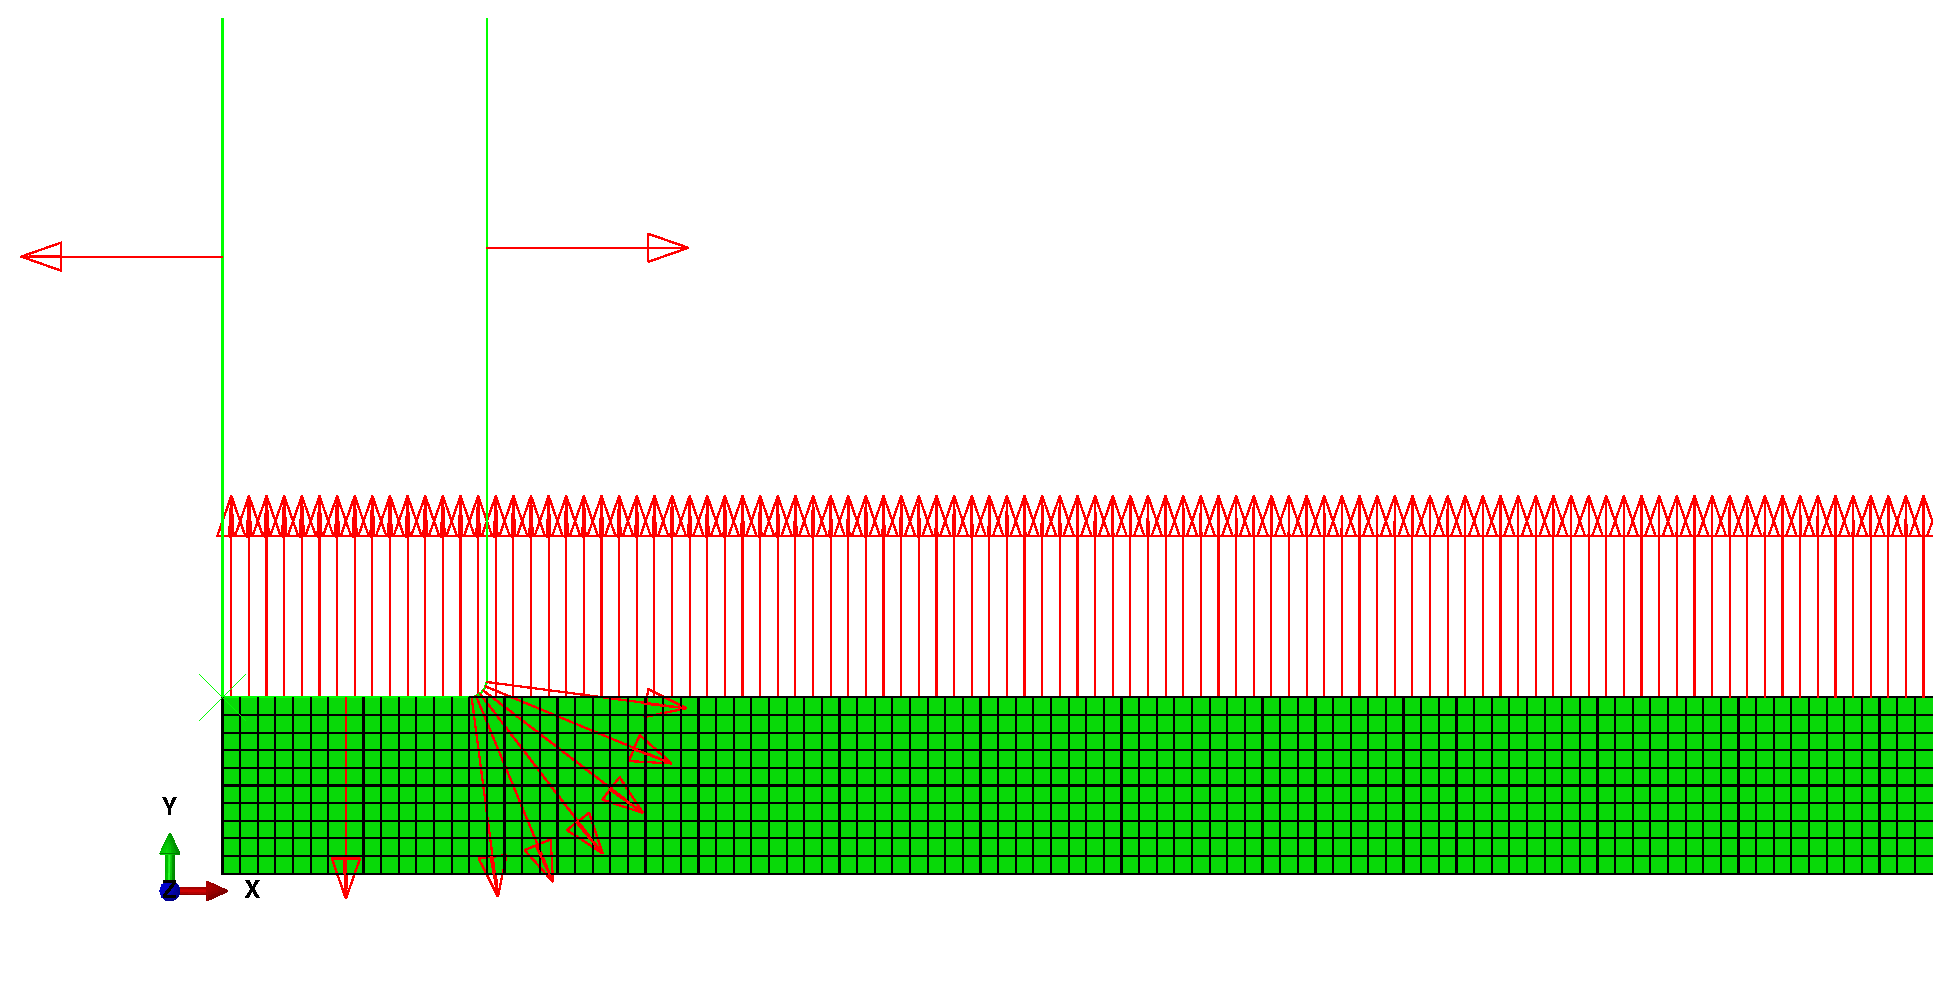
\includegraphics[trim={0cm 1cm 20cm 3.5cm},clip,width=0.4\linewidth]{pics/normals_corner}
    \caption{normals with a 1mm fillet}
  \end{subfigure}%
  \begin{subfigure}{.5\textwidth}
    \centering
    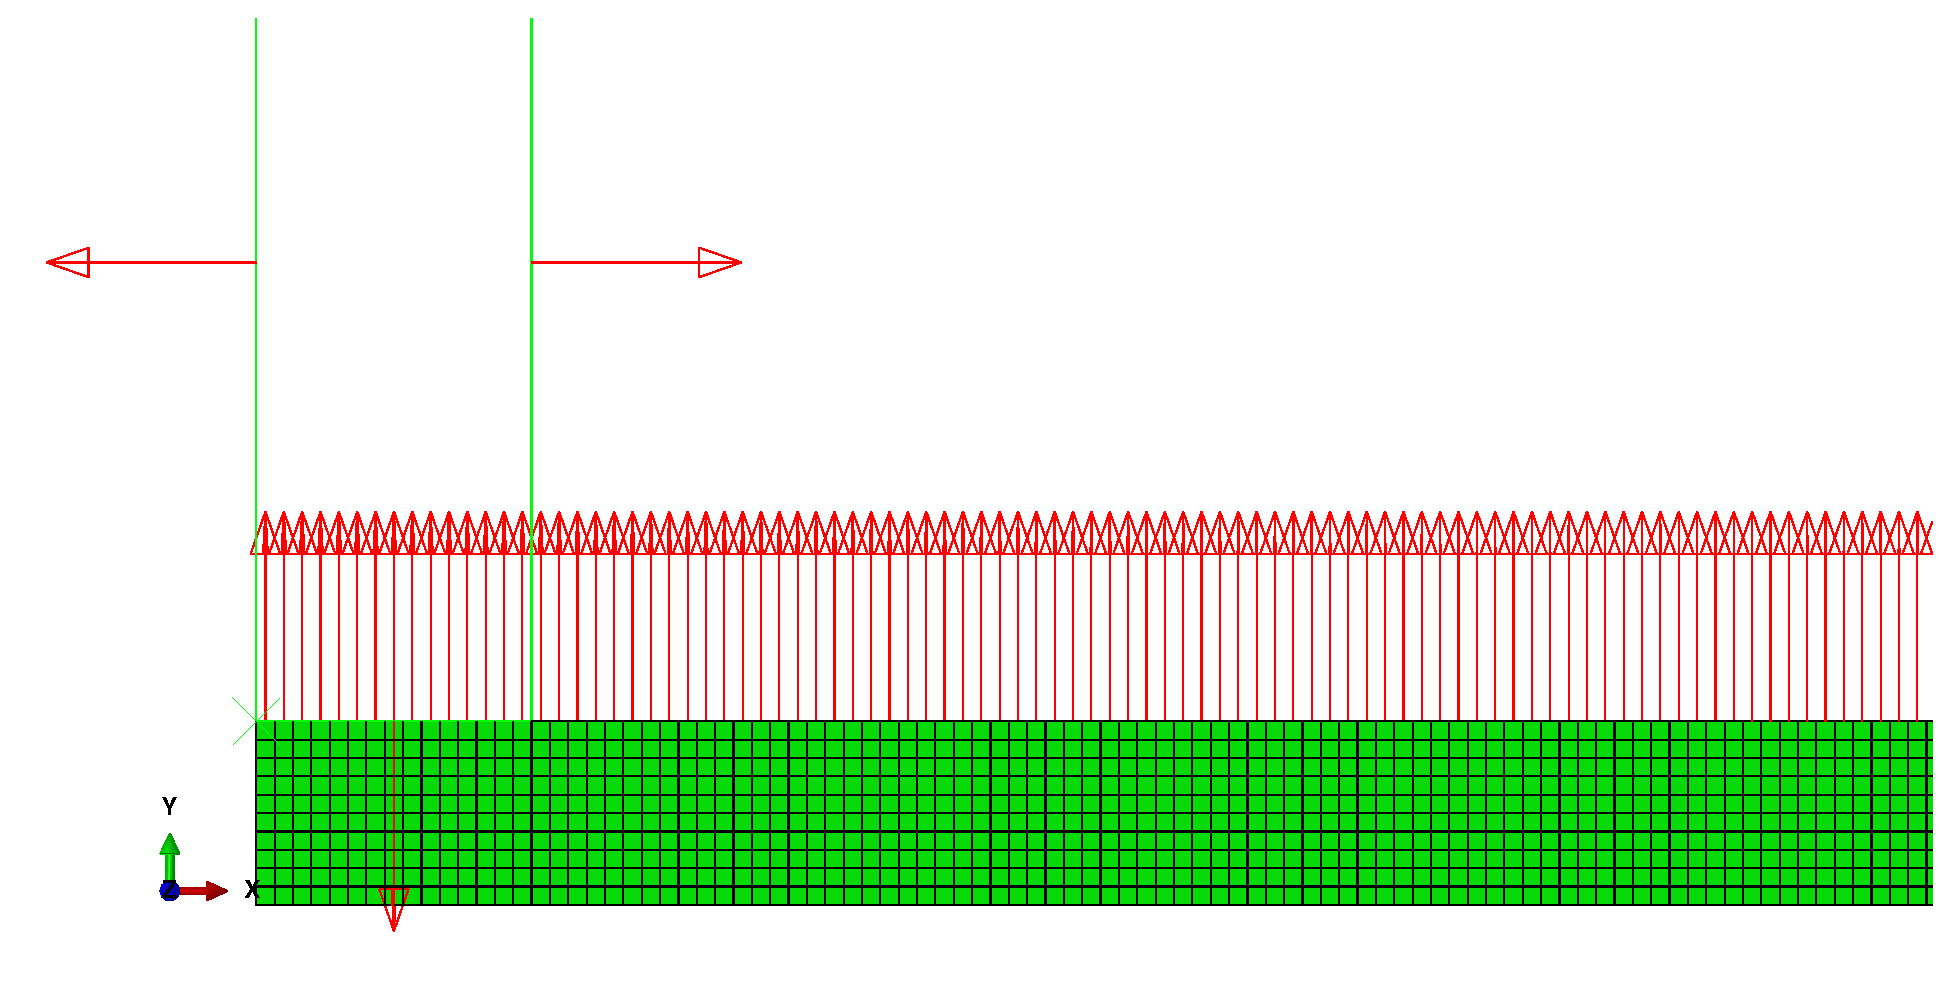
\includegraphics[trim={0cm 1cm 20cm 4cm},clip,width=0.4\linewidth]{pics/normals_no_corner}
    \caption{normals with no fillet}
   \end{subfigure}
  \caption{Comparsion of normals with fillet and no fillet}
  \label{fig:1}
\end{figure}
Figure 1 describes the relationship of the surface with the corresponding normals. Contact problems in Abaqus are hard to model as convergence problems can mess up the simulations. When a surface-to-surface approach is used, the discretization can lead to tangential motion in the salve surface in some cases. The motion can lead to unwanted effects and to the abortion of the report.
\begin{figure}[!htb]
  \centering
  \begin{subfigure}{.5\textwidth}
    \centering
    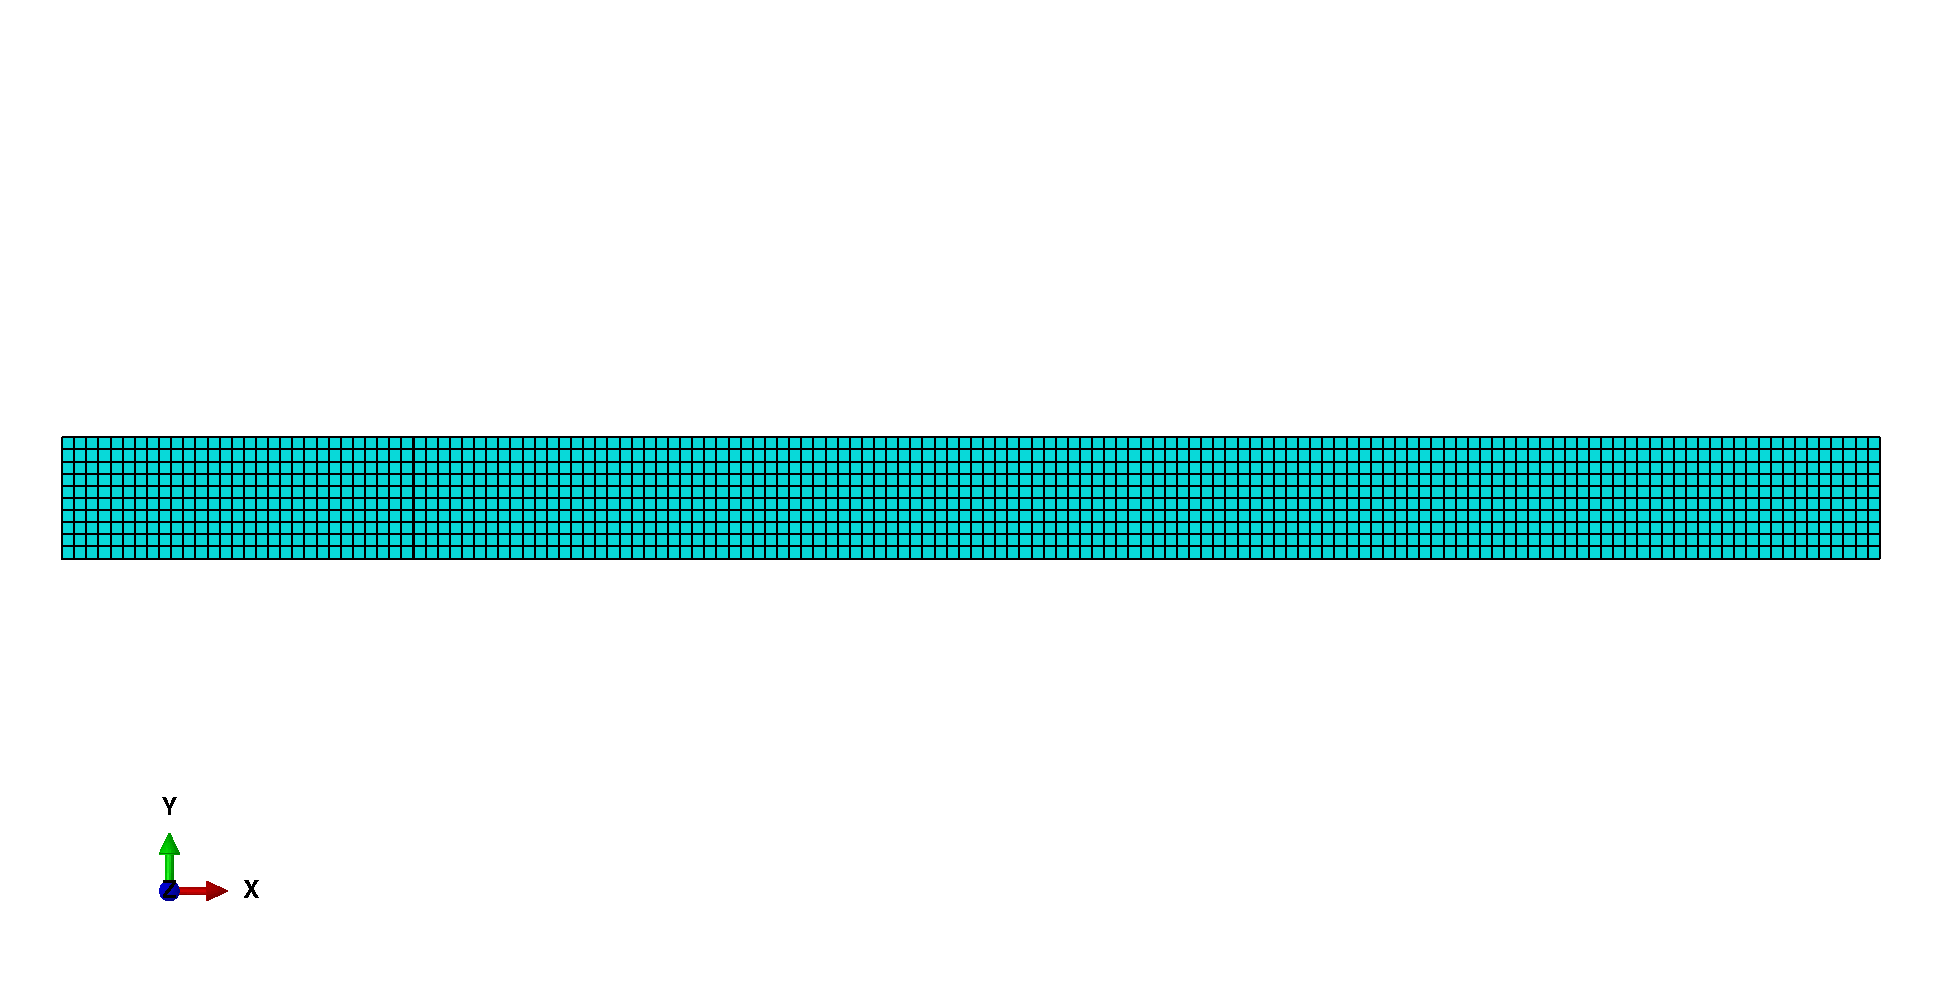
\includegraphics[trim={0cm 7cm 20cm 7cm},clip,width=0.7\linewidth]{pics/mesh_small}
    \caption{mesh with 1500 elements}
  \end{subfigure}%
  \begin{subfigure}{.5\textwidth}
    \centering
    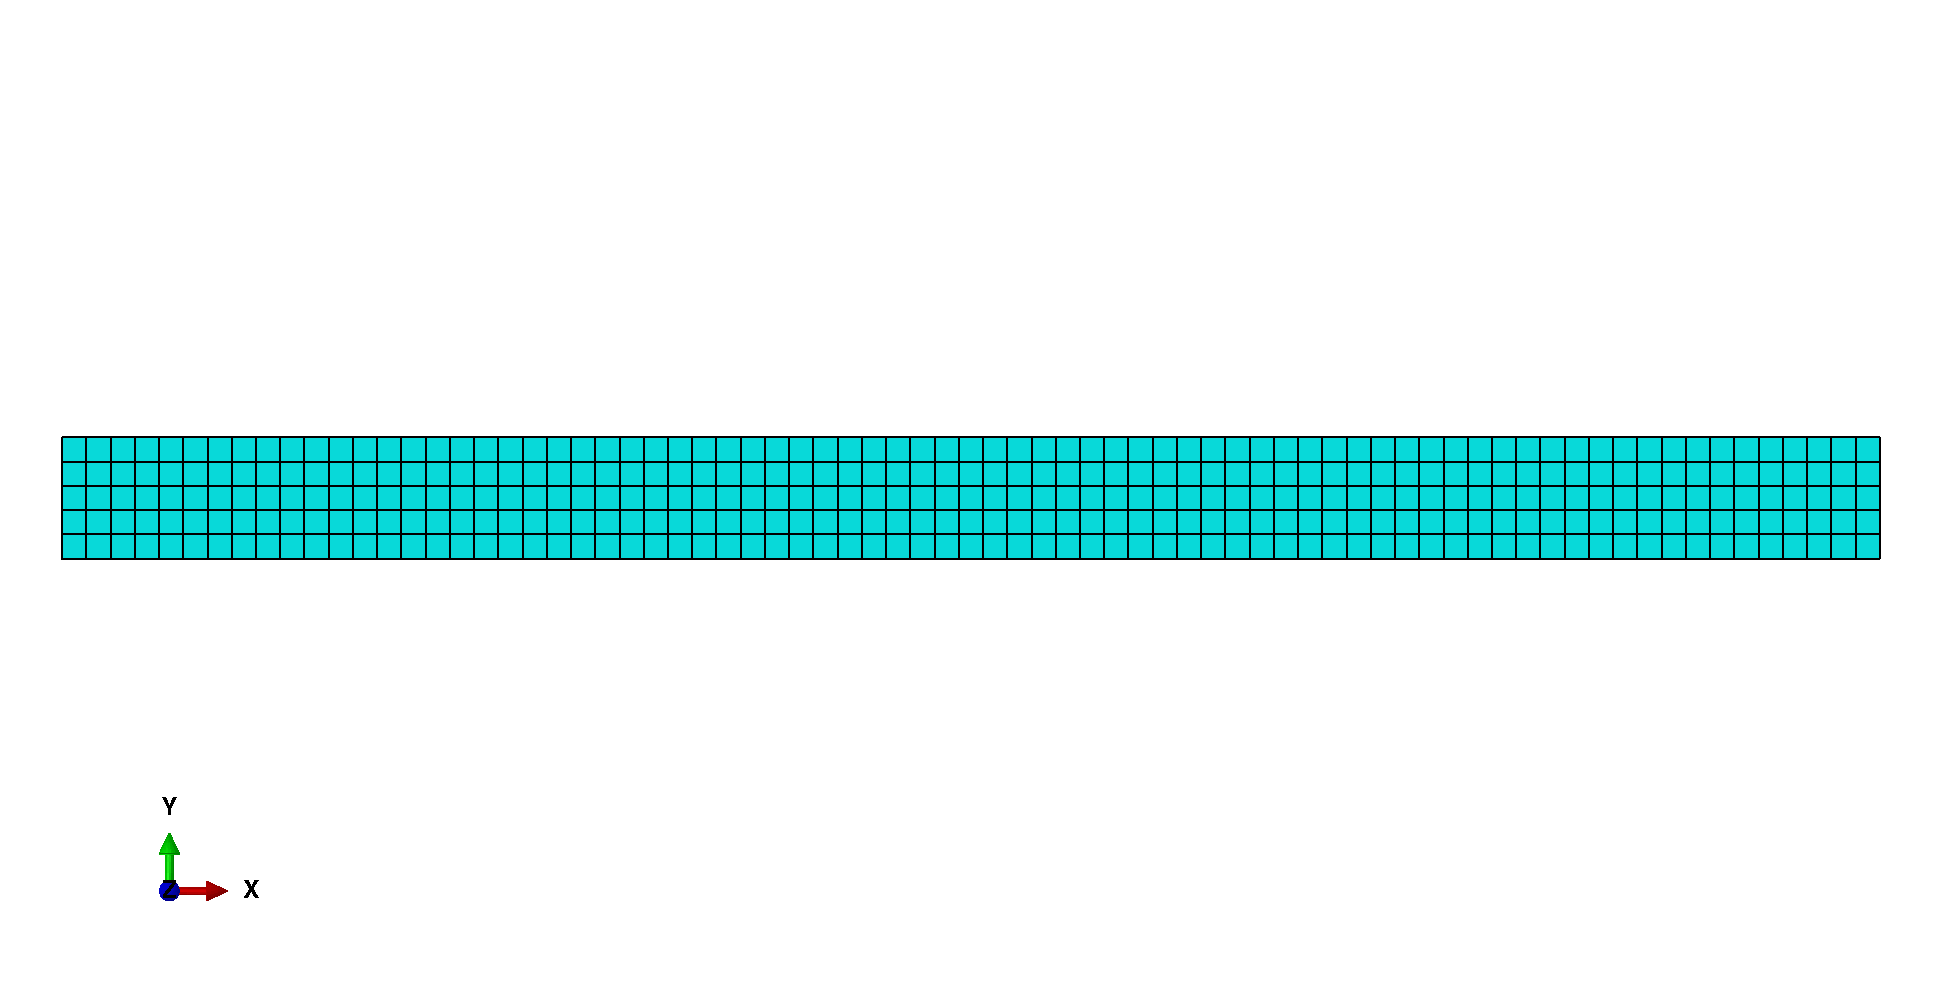
\includegraphics[trim={0cm 7cm 20cm 7cm},clip,width=0.7\linewidth]{pics/mesh_large}
    \caption{mesh with 375 elements}
   \end{subfigure}
  \caption{Global model with no fillet}
  \label{fig:2}
\end{figure}

The mesh size has an impact on the normals, regardless of the surface-to-surface or node-to-surface approach. So finding the correct mesh size is important for a successful job. With the running analysis, in each iteration, the nodes and surfaces are tracked when using small sliding. With finite sliding, the relationship with node and surfaces are established in every increment. So finite sliding is, therefore, more prone to failure of the job than small sliding, as it can stuck and loose itself.
\newpage

\section{Results}
The plots of the result are divided into no fillet and fillet. The frictionless approach is created using 1500 elements displayed in figure 2. The with friction approach was only successful with a smaller mesh size, resulting in a less apparent view of the sawtooth properties in the plot of the curve.
\begin{figure}[!htb]
  \centering
  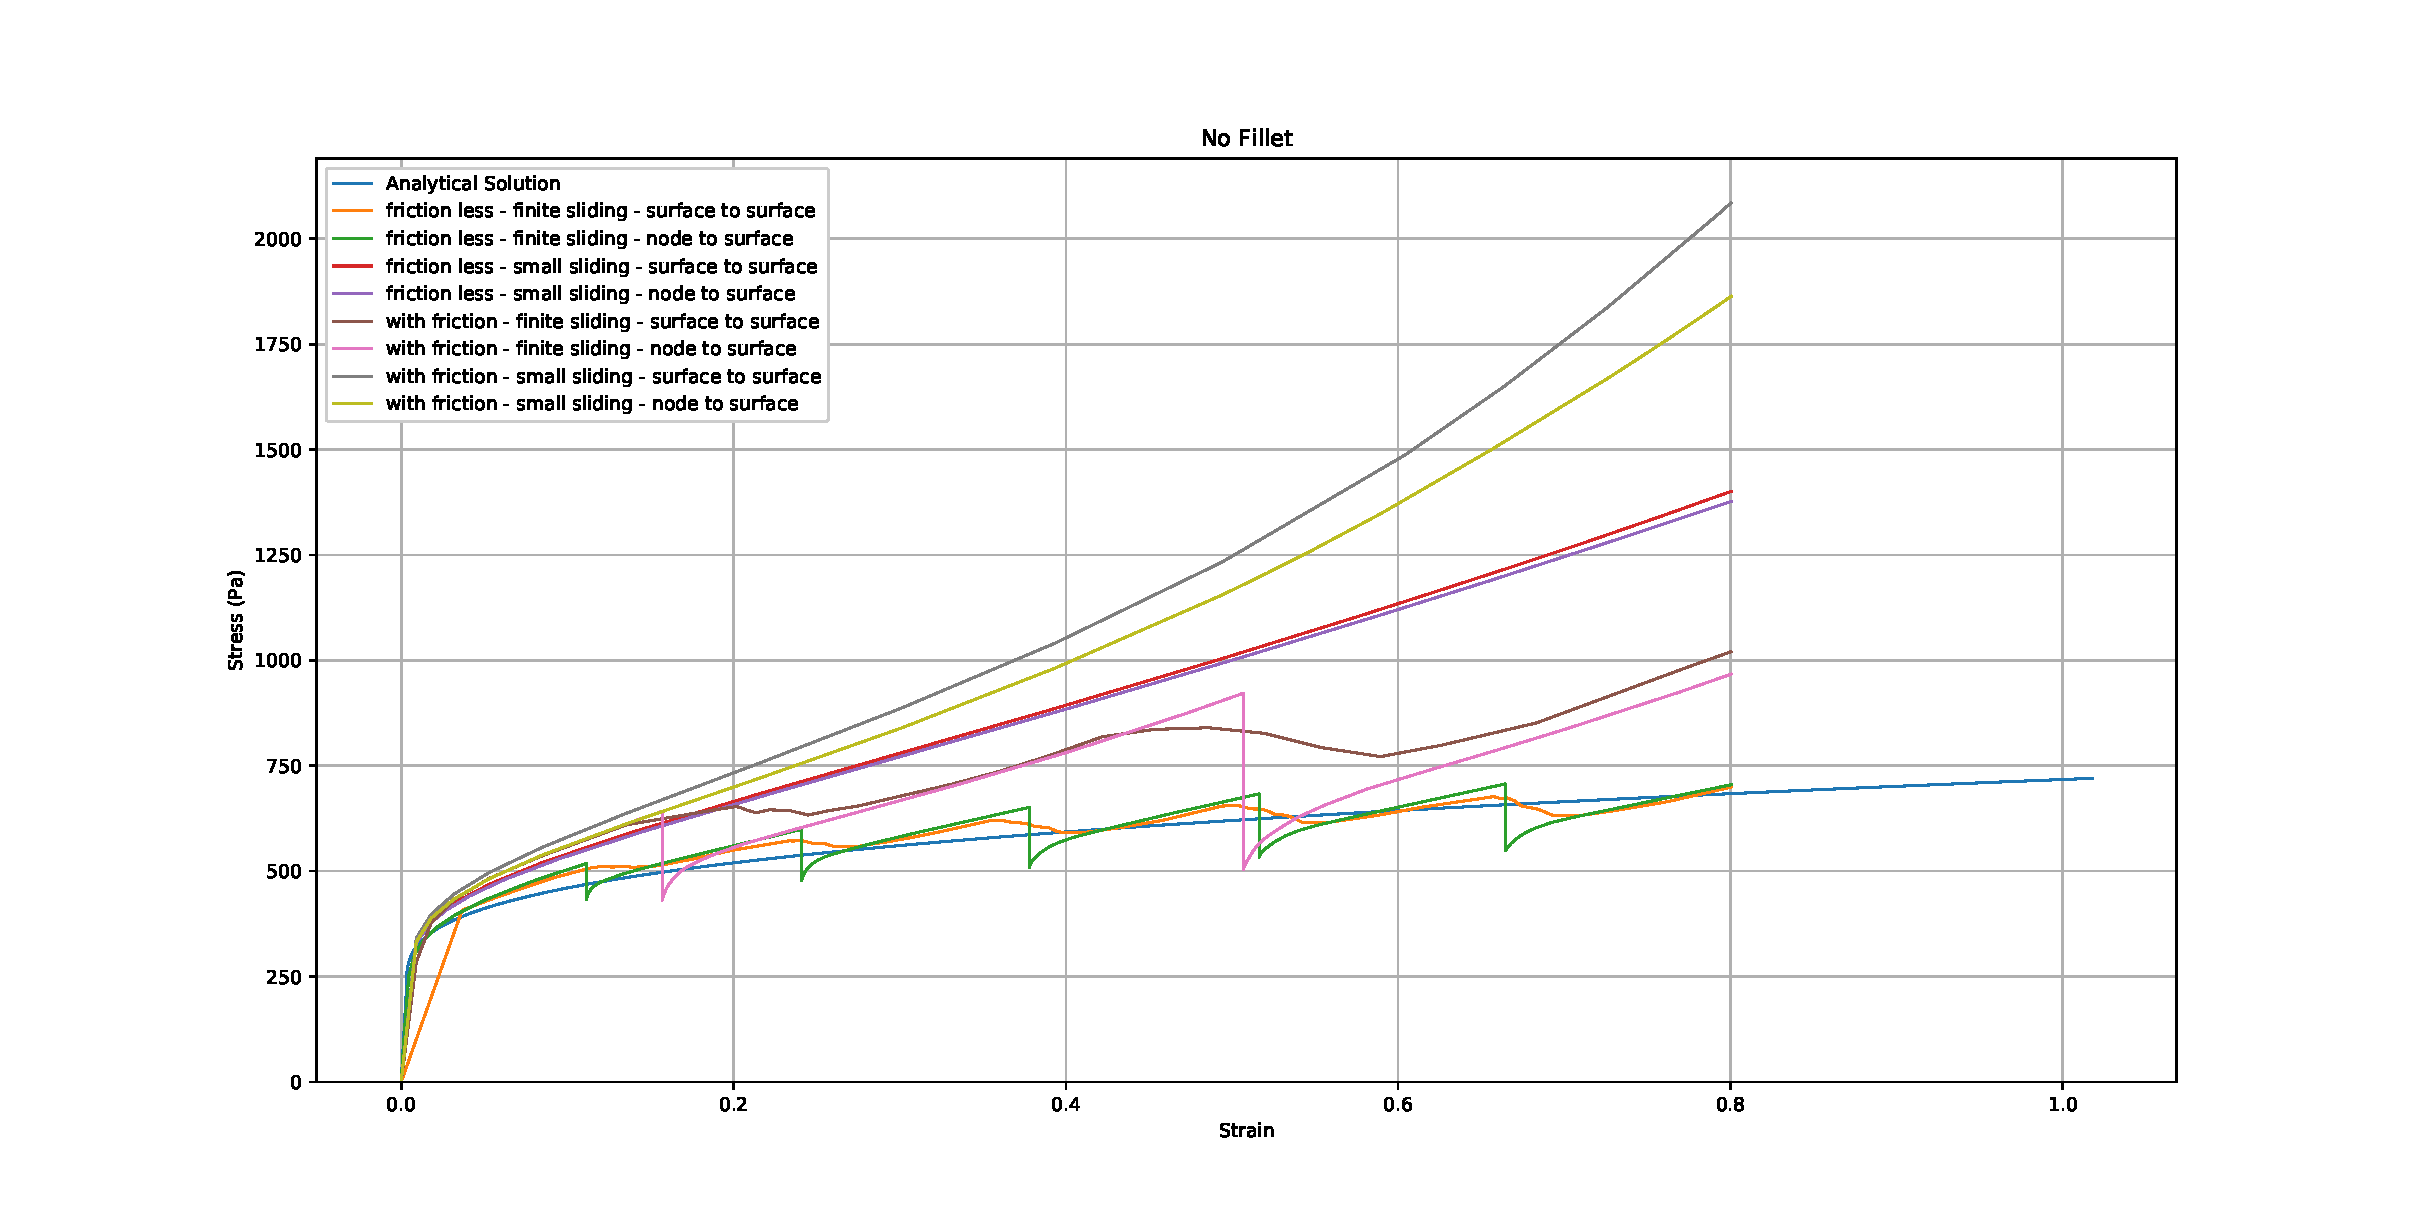
\includegraphics[trim={4cm 1cm 4cm 1.8cm},clip,width=0.9\linewidth]{pics/no_fillet}
  \caption{Results of the no fillet model}
  \label{fig:3}
\end{figure}

\begin{figure}[!htb]
  \centering
  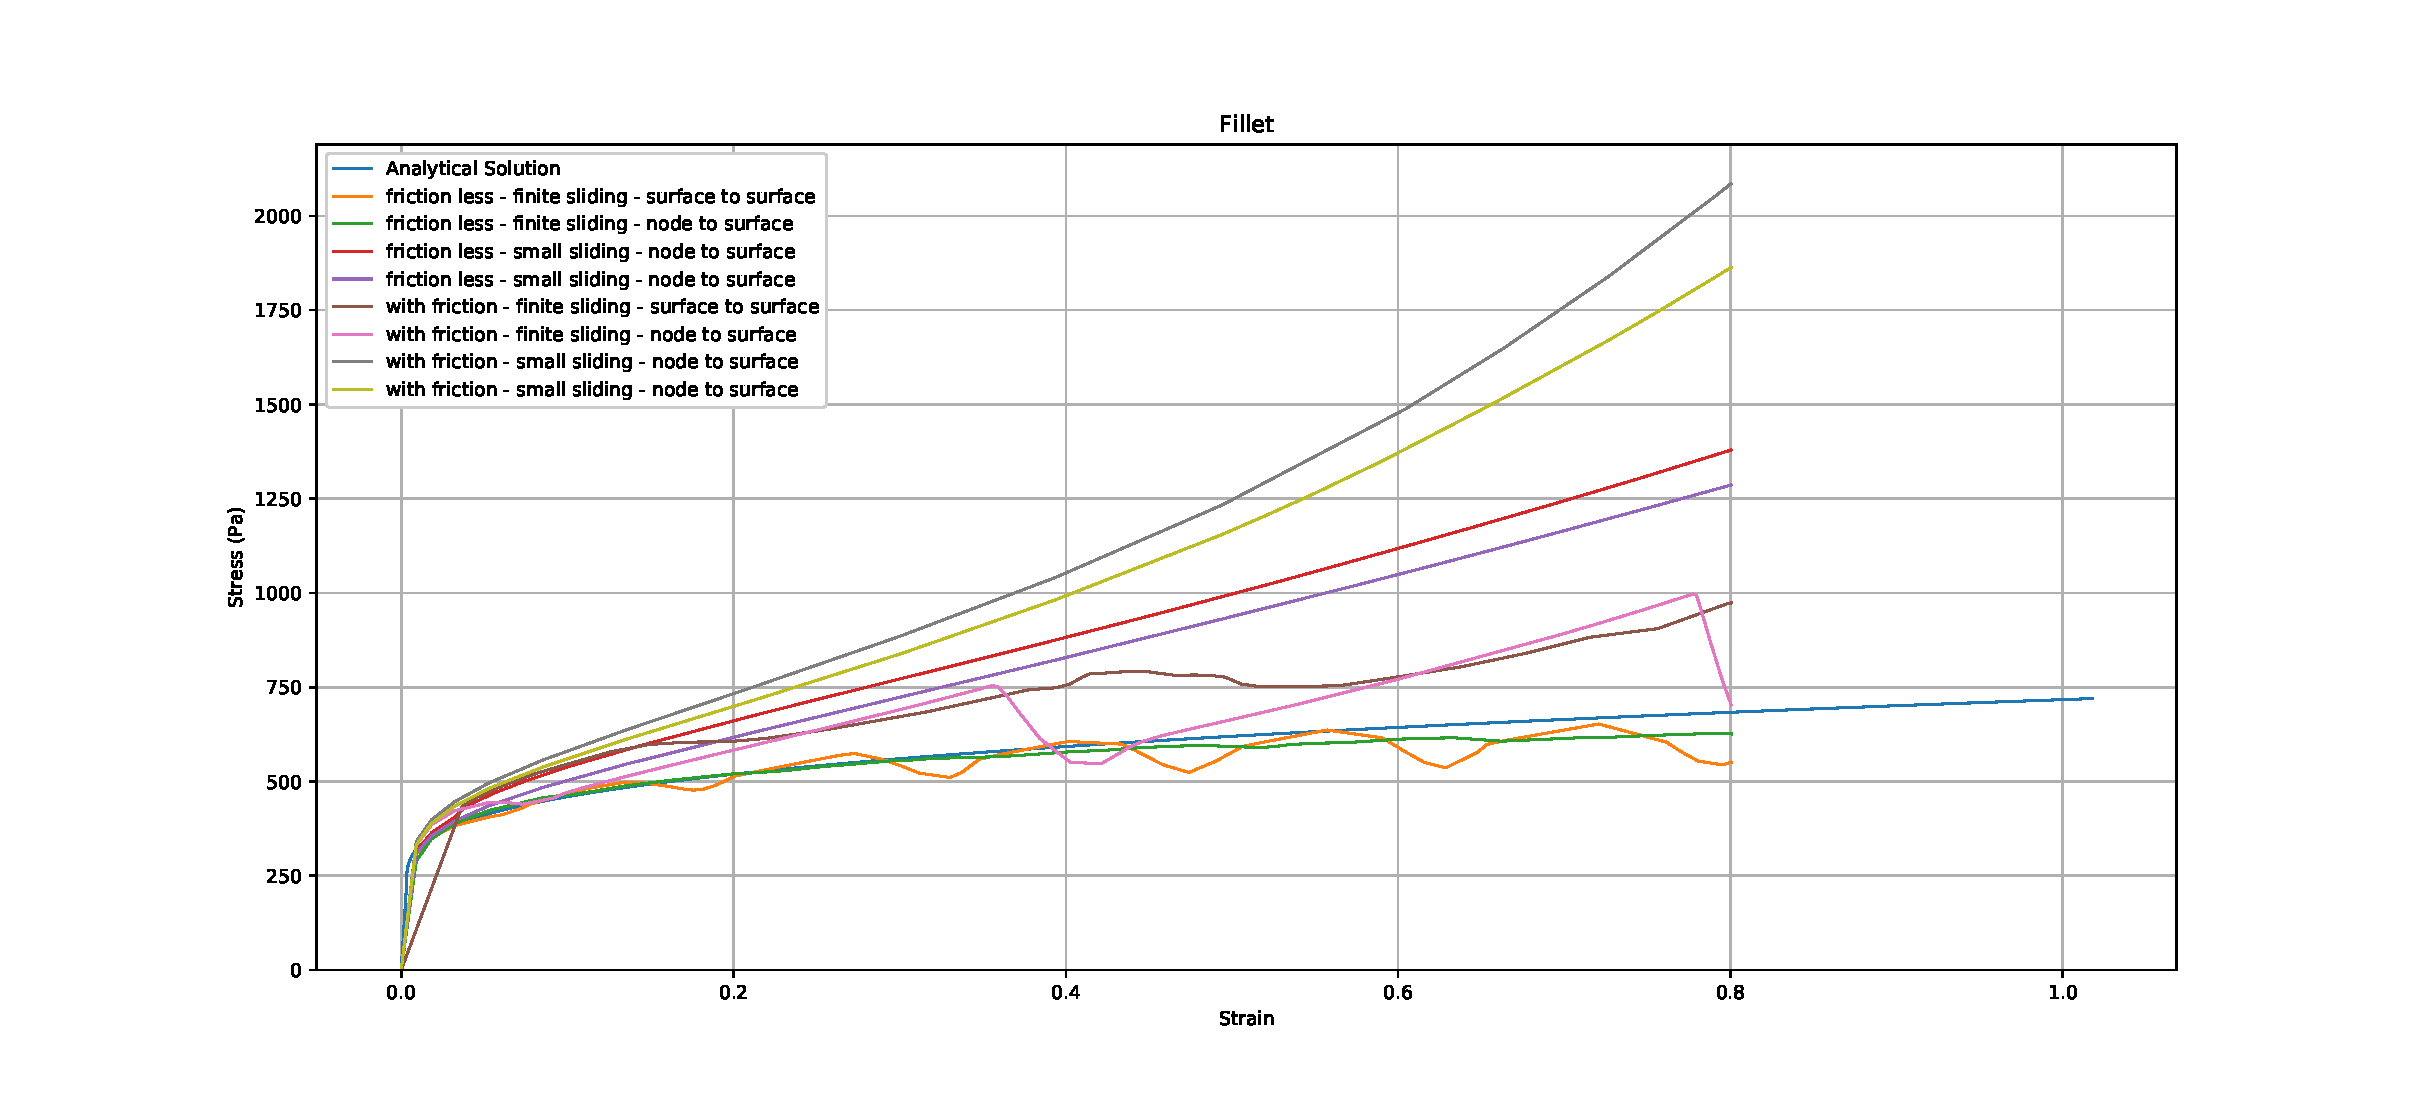
\includegraphics[trim={4cm 1cm 4cm 1.8cm},clip,width=0.9\linewidth]{pics/fillet}
  \caption{Results of the fillet model}
  \label{fig:4}
\end{figure}

\newpage

\section{Discussion}

\subsection{Surface to Surface}
The surface-to-surface method uses an average of the slave nodes nearby instead of individual slave nodes. This can also be seen in the curve as for the frictionless and finite sliding approach the surface-to-surface curve is much smoother in general. This discretization provides more accurate stress and pressure results compared to the node-to-surface approach
\subsection{Node to Surface}
With the node-to-surface method, the relationship between every slave node interacts with the closest master point. This approach simply resists penetrations of slave nodes into the master surface and the curve shows that by the good characteristic sawtooth properties of the curve.
\subsection{Finite sliding}
Finite sliding track the contact of the master and slave node in every incrementation. This leads to a large computational effort but to a more accurate solution.
\subsection{Small sliding}
Small sliding established the relationship between the nodes at the beginning of the analysis. This saves lots of computational time but also leading in a less accurate solution.
\subsection{Frictionless}
Usually, surfaces transmit shear and normal forces across the interface of the surfaces. The relationship between this to forces is called friction. The Frictionless behavior speaks for itself, not including this phenomenon into the analysis. Using no friction leads to a more equally distributed forces among the nodes and leads to a closer result to the analytical approach.
\subsection{With Friction}
With friction, the relationship between the shear and normal forces are taken into account. This leads in our case to a more inaccurate solution as the analytical version of the curve does not take this into account. The friction is an additional parameter which adds force to the interaction in the contact and so leads to a higher positive distance from the analytical curve.
\subsection{Fillet}
The fillet helps to smooth the surface. This adds more normals to the surface and leading to smoother output as can be seen in figure 4. 
\subsection{No Fillet}
With no filet, only one normal is present. The slave surface can only use one point in the masters surface. As the surface is not smoothed, the results are also more edged.
\subsection{Mesh and Thickness}
As previously mentioned the mesh size has an impact on the normals and so on the surfaces, nodes, and analysis. Creating a model which runs in every configuration is difficult. Increasing the mesh size leads to more accurate solutions but also the job is more likely to fail because many nodes are focusing on one master node in the no fillet approach. The convergence is also likely to fail. With the thickness, the force on the node can be distributed on the nodes. Either one can adjust the boundaries of the solver, or in our case, change the thickness for getting to a similar result.
\section{Conclusion}
Contact problems are rather difficult to model. Especially if one wants to implement a fillet in the model. Even the Abaqus documentation mentions that this approach is likely to fail, with the reasons mentioned above. For this appendix, the Abaqus documentations was used.

\end{document}